\documentclass[11pt,letterpaper]{article}

% CODIFICACIÓN E IDIOMA
\usepackage[utf8]{inputenc}     
\usepackage[T1]{fontenc}         % Salida de fuentes en T1: acentos y guionado correctos
\usepackage[spanish]{babel}      % Localización: "Tabla", "Figura", "Demostración", fechas, etc.
\decimalpoint
\usepackage{microtype}           % Micro-ajustes tipográficos (mejora notable de legibilidad)

% MATEMÁTICAS

\usepackage{amsmath,amssymb,amsfonts,amsthm}
\usepackage{mathtools}
\providecommand{\abs}[1]{\lvert#1\rvert}
\providecommand{\norm}[1]{\lVert#1\rVert}
\newcommand{\Aut}{\operatorname{Aut}}

% TIPOGRAFÍA

\usepackage{newpxtext,newpxmath}
\usepackage{titlesec}            % Formato de \section, \subsection, etc.

% GEOMETRÍA DE PÁGINA
\usepackage[a4paper,letterpaper,margin=2.5cm,headheight=14.5pt,includeheadfoot]{geometry}



% FIGURAS, TABLAS Y CÓDIGO

\usepackage{graphicx}
\graphicspath{{imagenes/}{figuras/}{img/}}
\usepackage{subcaption}          % Sustituye a "subfigure" (paquete obsoleto desde 2001)
\usepackage{caption}
\captionsetup{font=small,labelfont=bf,margin=8pt}
\usepackage{booktabs}            % Tablas profesionales (\toprule, \midrule, \bottomrule)
\usepackage{array}
\usepackage{siunitx}
% \sisetup{output-decimal-marker = {.}, group-separator = {,}}
% \sisetup{
%     locale = US,
%     output-decimal-marker = {.},
%     group-separator = {,}
% }
\usepackage{enumitem}            % Listas con espaciado controlado
\usepackage{listings}
\usepackage{xcolor}
\usepackage{tikz}
\usepackage{pgfplots}
\pgfplotsset{compat=1.18}        % Versión de compatibilidad actualizada (1.15 → 1.18)
\usetikzlibrary{arrows.meta}     % Sustituye a la librería "arrows", ya obsoleta


% ESPACIADO DE PÁRRAFOS
\setlength{\parindent}{0pt}
\setlength{\parskip}{0.65em plus 0.1em minus 0.1em}


% HIPERVÍNCULOS (se carga casi al final, como recomienda su documentación)
\usepackage{hyperref}
\hypersetup{
    colorlinks   = true,
    linkcolor    = {primary},
    citecolor    = {primary},
    urlcolor     = {primary!70!black},
    pdfborder    = {0 0 0},
    breaklinks   = true,
    bookmarksnumbered = true
}


% PALETA DE COLORES

\definecolor{primary}{RGB}{120,25,90}    % Vino/púrpura institucional (evolución de "purpura")
\definecolor{secondary}{RGB}{70,70,70}   % Gris oscuro para texto secundario
\definecolor{bgcode}{RGB}{247,247,250}   % Fondo suave para bloques de código
\hypersetup{linkcolor=primary, citecolor=primary, urlcolor=primary!70!black}

% TÍTULOS DE SECCIÓN 

\titleformat{\section}
  {\normalfont\Large\bfseries\sffamily\color{primary}}
  {\thesection}{0.8em}{}[{\color{primary!60}\titlerule[0.8pt]}]
\titlespacing*{\section}{0pt}{2.8ex plus 1ex minus .2ex}{1.4ex plus .2ex}

\titleformat{\subsection}
  {\normalfont\large\bfseries\sffamily\color{primary!85!black}}
  {\thesubsection}{0.8em}{}
\titlespacing*{\subsection}{0pt}{2.2ex plus 1ex minus .2ex}{1ex plus .2ex}

\titleformat{\subsubsection}
  {\normalfont\normalsize\bfseries\sffamily\color{secondary}}
  {\thesubsubsection}{0.8em}{}


% ENCABEZADO Y PIE DE PÁGINA

\usepackage{fancyhdr}
\pagestyle{fancy}
\fancyhf{}
\renewcommand{\headrulewidth}{0.6pt}
\renewcommand{\footrulewidth}{0.4pt}
\fancyheadoffset{0pt}

% Estilo "plain" (usado en la portada) sin encabezado
\fancypagestyle{plain}{%
  \fancyhf{}
  \renewcommand{\headrulewidth}{0pt}
  \renewcommand{\footrulewidth}{0pt}
}

% Datos del documento 
\newcommand{\asignaturaNombre}{Matemáticas}
\newcommand{\tareaNombre}{Tarea 1}
\newcommand{\autorNombre}{Eduardo Alanís García}
\newcommand{\institucionNombre}{MCDI}
\newcommand{\profesorNombre}{Dra. Briceyda B. Delgado López}
\newcommand{\fechaEntrega}{29 de agosto de 2026}


\fancyhead[L]{\small\color{primary}\textbf{\asignaturaNombre}}
\fancyhead[R]{\small\color{primary}\textbf{\tareaNombre}}
\fancyfoot[L]{\small\color{secondary}\autorNombre}
\fancyfoot[C]{\small\color{secondary}\thepage}
\fancyfoot[R]{\small\color{secondary}\institucionNombre}


% ENTORNOS TIPO TEOREMA
\newtheoremstyle{coloredplain}
  {0.9em}{0.9em}{\normalfont}{0pt}{\bfseries\color{primary}}{.}{0.6em}{}
\newtheoremstyle{coloreddef}
  {0.9em}{0.9em}{\normalfont}{0pt}{\bfseries\color{primary!75!black}}{.}{0.6em}{}

\theoremstyle{coloredplain}
\newtheorem{teorema}{Teorema}[section]
\newtheorem{lema}[teorema]{Lema}
\newtheorem{proposicion}[teorema]{Proposición}
\newtheorem{corolario}[teorema]{Corolario}

\theoremstyle{coloreddef}
\newtheorem{definicion}{Definición}[section]
\newtheorem{ejemplo}[definicion]{Ejemplo}
\newtheorem{observacion}[definicion]{Nota}
\newtheorem{afirmacion}[definicion]{Afirmación}
\newtheorem{pregunta}[definicion]{Pregunta}
\newtheorem{respuesta}[definicion]{Respuesta}
\newtheorem{ejercicio}{Ejercicio}


\renewcommand{\qedsymbol}{$\blacksquare$}
\newenvironment{solucion}
  {\par\noindent\textbf{\color{primary}Solución.}\ }
  %{\hfill$\blacksquare$\par}

\newenvironment{demostraccion}
  {\par\noindent\textbf{\color{primary}Demostración.}\ }
  {\hfill$\blacksquare$\par}

\newcommand{\pie}[1]{\footnote{#1}}


% CÓDIGO FUENTE (bloques "listings" con estilo unificado)

\lstdefinestyle{Rstyle}{
    language        = R,
    backgroundcolor = \color{bgcode},
    basicstyle      = \ttfamily\small,
    keywordstyle    = \color{primary}\bfseries,
    commentstyle    = \color{secondary}\itshape,
    stringstyle     = \color{teal},
    numbers         = left,
    numberstyle     = \tiny\color{secondary},
    numbersep       = 8pt,
    frame           = single,
    rulecolor       = \color{primary!30},
    breaklines      = true,
    showstringspaces= false,
    captionpos      = b,
    tabsize         = 2
}
\lstset{style=Rstyle}


% Referencias
\usepackage{csquotes}
\usepackage[numbers]{natbib}
% ============================================================================
\begin{document}


% PORTADA

\begin{titlepage}
  \thispagestyle{plain}
  \centering
  \vspace*{2.5cm}

  {\sffamily\color{secondary}\large Maestría en Ciencia de Datos e Información \par}
  \vspace{0.3cm}
  {\color{primary}\rule{0.5\textwidth}{0.8pt}\par}
  \vspace{2.2cm}

  {\sffamily\bfseries\color{primary}\Huge \tareaNombre \par}
  \vspace{0.6cm}
  {\sffamily\Large \asignaturaNombre \par}

  \vspace{3.5cm}
  {\color{primary!60}\rule{0.6\textwidth}{0.4pt}\par}
  \vspace{1cm}

  \begin{tabular}{rl}
    \textbf{Alumno:}   & \autorNombre \\[2pt]
    \textbf{Profesor:} & \profesorNombre \\[2pt]
    \textbf{Entrega:}    & \fechaEntrega \\
  \end{tabular}

  \vfill
  {\small\color{secondary} INFOTEC \par}
\end{titlepage}

% Descomente si desea un índice automático:
% \tableofcontents
% \newpage


\section*{Instrucciones}
Lea el archivo \emph{Formato de tareas} que se encuentra en la siguiente liga
\url{https://drive.google.com/drive/u/0/folders/1F-FI1J5PviBc-EPhfLbnE8PSvWnkgeHj}.
 
En la siguiente lista de ejercicios NO se admite ningún tipo de código en la
solución de los ejercicios, cada uno de ellos se puede resolver de forma
analítica. Párrafos que contengan código en la entrega no se van a considerar
en la calificación.

\section*{Ejercicios}

% EJERCICIO 1

\textbf{Herramientas utilizadas:} Todos los procedimientos, cálculos y verificaciones de esta tarea se realizaron de forma analítica y manual. El documento fue elaborado en LaTeX.


\begin{ejercicio}[15 puntos]
  Un inversionista le afirma a su corredor de bolsa que todas sus acciones
  pertenecen a tres compañías: Aeroméxico, Volaris y Vivaaerobus, y que hace
  dos días su valor bajó 350 pero que ayer aumentó 600. El corredor recuerda
  que hace dos días el precio de las acciones de Aeroméxico bajó 1 por cada
  una, mientras que las de Volaris bajaron 1.50, pero que el precio de las
  acciones de Vivaaerobus subió 0.50. También recuerda que ayer el precio de
  las acciones de Aeroméxico subió 1.50 por acción, el de las de Volaris bajó
  otros 0.50 por acción y las de Vivaaerobus subieron 1. Demuestre que el
  corredor no cuenta con la información suficiente para calcular el número de
  acciones que posee la inversionista en cada compañía, pero que si ella dice
  tener 280 acciones de Vivaaerobus, el corredor pueda calcular el número de
  acciones que posee en Aeroméxico y en Volaris.

  \begin{solucion}
    Sean $x_1$, $x_2$ y $x_3$ el número de acciones que la inversionista
    posee de Aeroméxico, Volaris y Vivaaerobus, respectivamente.

    \textbf{Hace dos días.} El precio de Aeroméxico bajó \$1 por acción, el
    de Volaris bajó \$1.50 por acción y el de Vivaaerobus subió \$0.50 por
    acción, mientras que el valor total del portafolio bajó \$350. Esto se
    escribe como
    \[
      -x_1-1.5\,x_2+0.5\,x_3=-350.
    \]

    \textbf{Ayer.} El precio de Aeroméxico subió \$1.50 por acción, el de
    Volaris bajó \$0.50 por acción y el de Vivaaerobus subió \$1 por acción,
    mientras que el valor total del portafolio subió \$600. Esto se escribe
    como
    \[
      1.5\,x_1-0.5\,x_2+x_3=600.
    \]

    Con esto, el sistema que describe la situación es
    \[
      \begin{cases}
        -x_1-1.5\,x_2+0.5\,x_3=-350,\\
        1.5\,x_1-0.5\,x_2+x_3=600.
      \end{cases}
    \]

    Este sistem tiene solo dos ecuaciones para tres incógnitas, así que antes de
    resolverlo ya podemos sospechar que no va a tener una única solución, ya que tiene ayor número de incógnitas que de ecuaciones. Resolviendo el sistema de ecuaciones por
    Gauss-Jordan:
    \[
    \begin{aligned}
    \left[
    \begin{array}{ccc|c}
    -1 & -1.5 & 0.5 & -350\\
    1.5 & -0.5 & 1 & 600
    \end{array}
    \right]
    &\xrightarrow{-R_1}
    \left[
    \begin{array}{ccc|c}
    1 & 1.5 & -0.5 & 350\\
    1.5 & -0.5 & 1 & 600
    \end{array}
    \right]
    \xrightarrow{R_2\leftarrow R_2-1.5R_1}
    \left[
    \begin{array}{ccc|c}
    1 & 1.5 & -0.5 & 350\\
    0 & -2.75 & 1.75 & 75
    \end{array}
    \right]\\[2ex]
    &\xrightarrow{-\frac{1}{2.75}R_2}
    \left[
    \begin{array}{ccc|c}
    1 & 1.5 & -0.5 & 350\\
    0 & 1 & -\frac{7}{11} & -\frac{300}{11}
    \end{array}
    \right]
    \xrightarrow{R_1\leftarrow R_1-1.5R_2}
    \left[
    \begin{array}{ccc|c}
    1 & 0 & \frac{5}{11} & \frac{4300}{11}\\
    0 & 1 & -\frac{7}{11} & -\frac{300}{11}
    \end{array}
    \right].
    \end{aligned}
    \]

    De esta manera notamos que, dejando $x_3=t$ como parámetro libre con
    $t\in\mathbb{R}$, el sistema queda descrito por
    \[
      x_1=\frac{4300-5t}{11},
      \qquad
      x_2=\frac{7t-300}{11},
      \qquad
      x_3=t.
    \]

    Es decir, por cada valor que elijamos para $x_3$ obtenemos una solución
    distinta $(x_1,x_2,x_3)$ que satisface las dos ecuaciones planteadas, todas ellas igualmente válidas. Como existen infinitas soluciones posibles, se demuestra que el corredor \emph{no} puede saber, únicamente con esta información, cuántas acciones tiene la inversionista en cada compañía.

    Supongamos ahora que la inversionista dice tener $x_3=280$ acciones de Vivaaerobus. Sustituyendo este valor en las dos ecuaciones originales, obtenemos
    \[
      -x_1-1.5x_2+0.5(280)=-350 \ \Longrightarrow\ x_1+1.5x_2=490,
    \]
    \[
      1.5x_1-0.5x_2+280=600 \ \Longrightarrow\ 1.5x_1-0.5x_2=320.
    \]

    A diferencia del caso anterior, ahora tenemos $2$ ecuaciones con $2$
    incógnitas, así que es de esperarse que exista una única solución.
    Resolvamos el sistema con Gauss-Jordan:
    \[
    \begin{aligned}
    \left[
    \begin{array}{cc|c}
    1 & 1.5 & 490\\
    1.5 & -0.5 & 320
    \end{array}
    \right]
    &\xrightarrow{R_2\leftarrow R_2-1.5R_1}
    \left[
    \begin{array}{cc|c}
    1 & 1.5 & 490\\
    0 & -2.75 & -415
    \end{array}
    \right]
    \xrightarrow{-\frac{1}{2.75}R_2}
    \left[
    \begin{array}{cc|c}
    1 & 1.5 & 490\\
    0 & 1 & \frac{1660}{11}
    \end{array}
    \right]\\[2ex]
    &\xrightarrow{R_1\leftarrow R_1-1.5R_2}
    \left[
    \begin{array}{cc|c}
    1 & 0 & \frac{2900}{11}\\
    0 & 1 & \frac{1660}{11}
    \end{array}
    \right].
    \end{aligned}
    \]

    De esta manera obtenemos directamente
    \[
      x_1=\frac{2900}{11}\approx 263.64,
      \qquad
      x_2=\frac{1660}{11}\approx 150.91.
    \]

    \textbf{Conclusión.} El
    sistema tiene dos ecuaciones y tres incógnitas, por lo que admite
    infinitas soluciones que dependen de un parámetro libre; por esta razón
    el corredor \emph{no} puede calcular por sí solo el número de acciones
    que la inversionista tiene en cada compañía. Sin embargo, si ella
    proporciona el dato adicional de que tiene $280$ acciones de
    Vivaaerobus, el sistema se reduce a dos ecuaciones con dos incógnitas
    con solución única, y el corredor sí puede calcular que ella posee
    \[
      x_1=\frac{2900}{11}\ \text{acciones de Aeroméxico}
      \qquad\text{y}\qquad
      x_2=\frac{1660}{11}\ \text{acciones de Volaris}.
    \]
  \end{solucion}
\end{ejercicio}

% EJERCICIO 2
\begin{ejercicio}[15 puntos]
  Considere el siguiente diagrama de una malla de calles de un sentido con
  vehículos que entran y salen de las intersecciones. La intersección $k$ se
  denota por $[k]$, $k=1,2,3,4$. Las flechas a lo largo de las calles indican
  la dirección del flujo del tráfico. Sea $x_i$ el número de vehículos que
  circulan por la calle $i$. Suponiendo que el tráfico que entra a una
  intersección también sale, establezca un sistema de ecuaciones que describa
  el diagrama del flujo de tráfico.

\begin{center}
    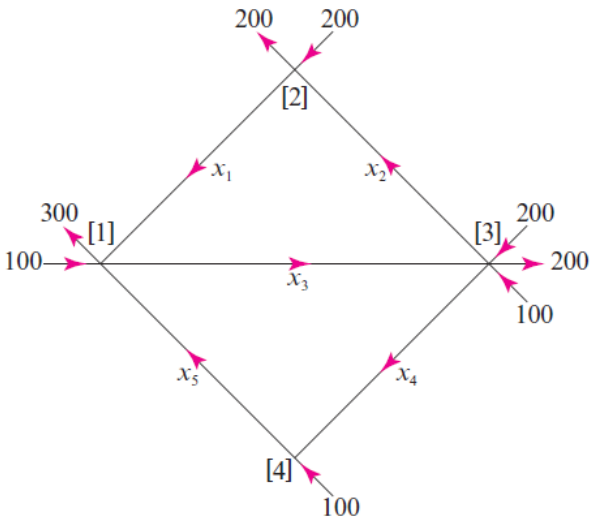
\includegraphics[width=0.5\textwidth]{Tarea 1 Figura Ejercicio 2}
\end{center}


  Por ejemplo, en la intersección $[1]$, la ecuación que lo representa es
  \[
    x_1 + x_5 + 100 = x_3 + 300.
  \]

  \begin{itemize}[leftmargin=1.4em]
    \item Proponga el sistema de ecuaciones que ilustra el flujo de tráfico
      de la imagen anterior.




      \begin{solucion}
          En la intersección $[1]$ entran $x_1$, $x_5$ y $100$ vehículos,
mientras que salen $x_3$ y $300$ vehículos. Por lo tanto,

\[
x_1+x_5+100=x_3+300.
\]

En la intersección $[2]$ entran $x_2$ y $200$ vehículos,
mientras que salen $x_1$ y $200$ vehículos. Por lo tanto,

\[
x_2+200=x_1+200.
\]

En la intersección $[3]$ entran $x_3$, $200$ y $100$ vehículos,
mientras que salen $x_2$, $x_4$ y $200$ vehículos. Por lo tanto,

\[
x_3+200+100=x_2+x_4+200.
\]

En la intersección $[4]$ entran $x_4$ y $100$ vehículos,
mientras que salen $x_5$ vehículos. Por lo tanto,

\[
x_4+100=x_5.
\]

De esta manera, el sistema de ecuaciones que representa el flujo de
tráfico en el diagrama es

\[
\begin{cases}
x_1+x_5+100=x_3+300,\\[2mm]
x_2+200=x_1+200,\\[2mm]
x_3+200+100=x_2+x_4+200,\\[2mm]
x_4+100=x_5.
\end{cases}
\]

Simplificando cada una de las ecuaciones, se obtiene

\[
\begin{cases}
x_1-x_3+x_5=200,\\
-x_1+x_2=0,\\
-x_2+x_3-x_4=-100,\\
-x_4+x_5=100.
\end{cases}
\]
      \end{solucion}



      
    \item Resuelva el sistema obtenido del flujo de tráfico.

    \begin{solucion}
      Partimos del sistema ya simplificado, escribimos la matriz aumentada, ordenando las incógnitas como
      $x_1,x_2,x_3,x_4,x_5$, y resolvemos por Gauss-Jordan:
\[
\begin{aligned}
&\left[
\begin{array}{ccccc|c}
1 & 0 & -1 & 0 & 1 & 200\\
-1 & 1 & 0 & 0 & 0 & 0\\
0 & -1 & 1 & -1 & 0 & -100\\
0 & 0 & 0 & -1 & 1 & 100
\end{array}
\right]
\xrightarrow{\;R_2\leftarrow R_2+R_1\;}
\left[
\begin{array}{ccccc|c}
1 & 0 & -1 & 0 & 1 & 200\\
0 & 1 & -1 & 0 & 1 & 200\\
0 & -1 & 1 & -1 & 0 & -100\\
0 & 0 & 0 & -1 & 1 & 100
\end{array}
\right]
\\[3ex]
&\hspace{7em}
\xrightarrow{\;R_3\leftarrow R_3+R_2\;}
\left[
\begin{array}{ccccc|c}
1 & 0 & -1 & 0 & 1 & 200\\
0 & 1 & -1 & 0 & 1 & 200\\
0 & 0 & 0 & -1 & 1 & 100\\
0 & 0 & 0 & -1 & 1 & 100
\end{array}
\right]
\xrightarrow{\;R_4\leftarrow R_4-R_3\;}
\left[
\begin{array}{ccccc|c}
1 & 0 & -1 & 0 & 1 & 200\\
0 & 1 & -1 & 0 & 1 & 200\\
0 & 0 & 0 & -1 & 1 & 100\\
0 & 0 & 0 & 0 & 0 & 0
\end{array}
\right]
\\[3ex]
&\hspace{7em}
\xrightarrow{\;-R_3\;}
\left[
\begin{array}{ccccc|c}
1 & 0 & -1 & 0 & 1 & 200\\
0 & 1 & -1 & 0 & 1 & 200\\
0 & 0 & 0 & 1 & -1 & -100\\
0 & 0 & 0 & 0 & 0 & 0
\end{array}
\right].
\end{aligned}
\]

De esta manera nuestro sistema es:

\[
\begin{cases}
x_1-x_3+x_5=200,\\
x_2 - x_3 + x_5=200,\\
x_4 - x_5= -100.
\end{cases} 
\Longrightarrow
\begin{cases}
x_1= 200 + x_3 - x_5,\\
x_2 =200 + x_3 - x_5,\\
x_4 = -100 + x_5
\end{cases} 
\] 

      Por lo tanto, la solución general del sistema de flujo de tráfico es
      \[
        \begin{pmatrix}
          x_1\\ x_2\\ x_3\\ x_4\\ x_5
        \end{pmatrix}
        =
        \begin{pmatrix}
          200+  x_3 - x_5\\
          200+  x_3 - x_5\\
          x_3\\
          -100 + x_5\\
          x_5
        \end{pmatrix} =
        \begin{pmatrix}
          200 \\
          200 \\
          0\\
          -100 \\
          0
        \end{pmatrix} +
        x_3
        \begin{pmatrix}
          1 \\
          1 \\
          1\\
          0 \\
          0
        \end{pmatrix} +
        x_5
        \begin{pmatrix}
          -1 \\
          -1 \\
          0\\
          1 \\
          1
        \end{pmatrix} 
      \]

      donde $x_3$ y $x_5$ son parámetros libres que representan el
      flujo vehicular en las calles de $[1]$ a $[3]$ y de $[4]$ a $[1]$.
    \end{solucion}


    
    \item Suponga que la calle de $[1]$ a $[3]$ necesita cerrarse; es decir,
      $x_3 = 0$. ¿Puede cerrarse también la calle de $[1]$ a $[4]$, es decir
      $x_5 = 0$ sin modificar los sentidos del tránsito? Si no se puede
      cerrar ¿cuál es la cantidad más pequeña de vehículos que debe poder
      admitir esta calle (de $[1]$ a $[4]$)?



       \begin{solucion}
        De la solución general obtenida en el inciso anterior, al suponer
        $x_3=0$ obtenemos.
        \[
        \begin{pmatrix}
          x_1\\ x_2\\ x_3\\ x_4\\ x_5
        \end{pmatrix} =
        \begin{pmatrix}
          200 \\
          200 \\
          0\\
          -100 \\
          0
        \end{pmatrix} +
        x_5
        \begin{pmatrix}
          -1 \\
          -1 \\
          0\\
          1 \\
          1
        \end{pmatrix} 
        \]

        Cada $x_i$ debe cumplir
        $x_i \geq 0$ para $i=1,2,3,4,5$. Un valor negativo significaría
        tráfico circulando en sentido contrario al indicado, lo cual no está
        permitido. Esto impone las siguientes restricciones sobre $x_5$:
        \begin{itemize}
          \item De $x_1 = 200 - x_5 \geq 0$ se
            obtiene $x_5 \leq 200$.
          \item De $x_2 = 200 - x_5 \geq 0$ se
            obtiene $x_5 \leq 200$.
          \item De $x_4 = -100 + x_5 \geq 0$ se
            obtiene $x_5 \geq 100$.
        \end{itemize}
        Asi
        \[
          100 \leq x_5 \leq 200.
        \]

        \medskip
        \noindent\textbf{¿Se puede cerrar también la calle de $[1]$ a $[4]$?}
        Cerrar dicha calle equivale a pedir $x_5 = 0$. Como $0$ no
        pertenece al intervalo $[100,200]$ obtenido, la respuesta es
        \textbf{no}: no es posible cerrar simultáneamente la calle de $[1]$
        a $[3]$ y la calle de $[1]$ a $[4]$ sin modificar los sentidos del
        tránsito.
        
        \textbf{Cantidad mínima de vehículos que debe admitir la
        calle de $[1]$ a $[4]$.} Puesto que $x_5$ debe satisfacer
        $100\leq x_5\leq 200$, el valor más pequeño posible es
        \[
          x_5 = 100.
        \]
        Es decir, si se cierra la calle de $[1]$ a $[3]$, la calle de $[4]$
        a $[1]$ debe poder admitir \textbf{al menos $100$ vehículos} para
        que el sistema siga siendo consistente con los sentidos de
        circulación indicados en el diagrama. En este caso extremo
        ($x_5=100$), la solución completa del sistema es
        \[
          x_1 = 100, \qquad x_2 = 100, \qquad x_3 = 0, \qquad
          x_4 = 0, \qquad x_5 = 100,
        \]
        donde, en particular, $x_4=0$ significa que en este escenario
        límite la calle de $[3]$ a $[4]$ tampoco tendría flujo vehicular:
        todo el flujo externo que entra en $[4]$ ($100$ vehículos) sale
        íntegramente por la calle $x_5$ hacia $[1]$.
      \end{solucion}
  \end{itemize}

  
\end{ejercicio}

% EJERCICIO 3
\begin{ejercicio}[20 puntos]
  Utilice la inversa de matrices para codificar un mensaje asignado en clase
  de forma personalizada. Se utilizará arreglos de tamaño 3 y la siguiente
  matriz de $3\times 3$
  \[
    A =
    \begin{pmatrix}
      2 & 4 & 3 \\
      0 & 1 & -1 \\
      3 & 5 & 7
    \end{pmatrix}
  \]

  Cada letra del mensaje a encriptar será representada por un número módulo
  26.

  \begin{center}
    \renewcommand{\arraystretch}{1.2}
    \begin{tabular}{|c|c c c c c c c c c c c c c|}
      \hline
      Letter & A & B & C & D & E & F & G & H & I & J & K & L & M \\
      Number & 1 & 2 & 3 & 4 & 5 & 6 & 7 & 8 & 9 & 10 & 11 & 12 & 13 \\
      \hline
    \end{tabular}

    \vspace{0.5em}

    \begin{tabular}{|c|c c c c c c c c c c c c c|}
      \hline
      Letter & N & O & P & Q & R & S & T & U & V & W & X & Y & Z \\
      Number & 14 & 15 & 16 & 17 & 18 & 19 & 20 & 21 & 22 & 23 & 24 & 25 & 0 \\
      \hline
    \end{tabular}
  \end{center}

  Explique paso a paso el proceso de encriptado y desencriptado del mensaje.

  \begin{solucion}

  El mensaje personalizado a codificar es:

  
  \textbf{En un lugar de la Mancha, de cuyo nombre no quiero acordarme, no hace mucho tiempo que vivía un hidalgo.}

  El procedimiento consiste en transformar cada letra del mensaje en un número, agrupar esos números en vectores de tamaño 3 y multiplicar cada vector por la matriz $A$, trabajando siempre módulo 26, para obtener el mensaje cifrado. Para recuperar el mensaje a partir del texto cifrado se realiza el proceso inverso: se multiplica cada vector cifrado por $A^{-1}$ en lugar de por $A$.

  Puesto que la tabla de conversión solo contempla las 26 letras del alfabeto, antes de codificar se eliminan los espacios, los signos de puntuación y los acentos, obteniendo el siguiente texto:

  \begin{center}
  \textbf{ENUNLUGARDELAMANCHADECUYONOMBRENOQUIEROACORDARMENOHACE}
  
  \textbf{MUCHOTIEMPOQUEVIVIAUNHIDALGO}
  \end{center}
  

  
  Este texto tiene 82 letras. Como $82=3(27)+1$, la cantidad de letras no es múltiplo de 3, así que se agregan 2 letras de relleno al final. Se elige la letra \textbf{X}, que simplemente se descartará al terminar de descifrar. Con esto el mensaje queda de 84 letras, es decir, se forman 28 bloques de tamaño 3.

  \subsection*{Parte 1: Codificación (encriptado)}

  \textbf{Paso 1: convertir las letras en números.}
  Usando la tabla dada, cada letra del mensaje con relleno se traduce a su número correspondiente y se agrupa en
  vectores columna de tamaño 3, respetando el orden en que aparecen en el texto.

  \textbf{Paso 2: multiplicar cada vector por $A$ y reducir módulo 26.}
  La regla de cifrado es $Av \pmod{26}$. A modo de ejemplo, se muestra el
  procedimiento completo para el primer bloque, \textbf{ENU} $\to
  (5,14,21)^t$:
  \begin{align*}
    Av_1
    &=
    \begin{pmatrix}2&4&3\\0&1&-1\\3&5&7\end{pmatrix}
    \begin{pmatrix}5\\14\\21\end{pmatrix}
    =
    \begin{pmatrix}
      2(5)+4(14)+3(21)\\
      0(5)+1(14)-1(21)\\
      3(5)+5(14)+7(21)
    \end{pmatrix}
    =
    \begin{pmatrix}129\\-7\\232\end{pmatrix} \\[1ex]
    &\equiv \begin{pmatrix}25\\19\\24\end{pmatrix}\pmod{26}
    \ \longrightarrow\ \text{Y, S, X},
  \end{align*}
  ya que $129=4(26)+25$, $-7\equiv -7+26=19$, y $232=8(26)+24$.

  Los 27 bloques restantes se calculan siguiendo exactamente el mismo procedimiento; solo cambian los valores de entrada. 

  \begin{center}
    \renewcommand{\arraystretch}{1.15}
    \small
    \begin{tabular}{|c|c|c|c|c|c|}
      \hline
      \# & Letras & $v$ & $Av$ (sin reducir) & $Av \bmod 26$ & Cifrado \\
      \hline
      1  & ENU & (5,14,21)  & (129,-7,232)   & (25,19,24) & YSX \\
      2  & NLU & (14,12,21) & (139,-9,249)   & (9,17,15)  & IQO \\
      3  & GAR & (7,1,18)   & (72,-17,152)   & (20,9,22)  & TIV \\
      4  & DEL & (4,5,12)   & (64,-7,121)    & (12,19,17) & LSQ \\
      5  & AMA & (1,13,1)   & (57,12,75)     & (5,12,23)  & ELW \\
      6  & NCH & (14,3,8)   & (64,-5,113)    & (12,21,9)  & LUI \\
      7  & ADE & (1,4,5)    & (33,-1,58)     & (7,25,6)   & GYF \\
      8  & CUY & (3,21,25)  & (165,-4,289)   & (9,22,3)   & IVC \\
      9  & ONO & (15,14,15) & (131,-1,220)   & (1,25,12)  & AYL \\
      10 & MBR & (13,2,18)  & (88,-16,175)   & (10,10,19) & JJS \\
      11 & ENO & (5,14,15)  & (111,-1,190)   & (7,25,8)   & GYH \\
      12 & QUI & (17,21,9)  & (145,12,219)   & (15,12,11) & OLK \\
      13 & ERO & (5,18,15)  & (127,3,210)    & (23,3,2)   & WCB \\
      14 & ACO & (1,3,15)   & (59,-12,123)   & (7,14,19)  & GNS \\
      15 & RDA & (18,4,1)   & (55,3,81)      & (3,3,3)    & CCC \\
      16 & RME & (18,13,5)  & (103,8,154)    & (25,8,24)  & YHX \\
      17 & NOH & (14,15,8)  & (112,7,173)    & (8,7,17)   & HGQ \\
      18 & ACE & (1,3,5)    & (29,-2,53)     & (3,24,1)   & CXA \\
      19 & MUC & (13,21,3)  & (119,18,165)   & (15,18,9)  & ORI \\
      20 & HOT & (8,15,20)  & (136,-5,239)   & (6,21,5)   & FUE \\
      21 & IEM & (9,5,13)   & (77,-8,143)    & (25,18,13) & YRM \\
      22 & POQ & (16,15,17) & (143,-2,242)   & (13,24,8)  & MXH \\
      23 & UEV & (21,5,22)  & (128,-17,242)  & (24,9,8)   & XIH \\
      24 & IVI & (9,22,9)   & (133,13,200)   & (3,13,18)  & CMR \\
      25 & AUN & (1,21,14)  & (128,7,206)    & (24,7,24)  & XGX \\
      26 & HID & (8,9,4)    & (64,5,97)      & (12,5,19)  & LES \\
      27 & ALG & (1,12,7)   & (71,5,112)     & (19,5,8)   & SEH \\
      28 & OXX & (15,24,24) & (198,0,333)    & (16,0,21)  & PZU \\
      \hline
    \end{tabular}
  \end{center}

  Uniendo los 28 bloques cifrados, el mensaje encriptado es:



\begin{center}
\textbf{YSXIQOTIVLSQELWLUIGYFIVCAYLJJSGYHOLKWCBGNSCCCYHXHGQCXAORIFUE}

\textbf{YRMMXHXIHCMRXGXLESSEHPZU}
\end{center}



  \subsection*{Parte 2: Decodificación (desencriptado)}

  Para descifrar es necesario "deshacer" la multiplicación por $A$, así
  que se calcula la inversa $A^{-1}$ y se usa para recuperar los vectores
  originales a partir del mensaje cifrado.

  \textbf{Paso 1: calcular $A^{-1}$ con eliminación de Gauss-Jordan.}
  Se construye la matriz aumentada $[A\mid I]$ y se aplican operaciones
  por fila hasta que el bloque izquierdo se convierta en la identidad.

  \[
  \begin{aligned}
  \left[
  \begin{array}{ccc|ccc}
  2 & 4 & 3 & 1 & 0 & 0\\
  0 & 1 & -1 & 0 & 1 & 0\\
  3 & 5 & 7 & 0 & 0 & 1
  \end{array}
  \right]
  &\xrightarrow{\frac{1}{2}R_1}
  \left[
  \begin{array}{ccc|ccc}
  1 & 2 & \frac{3}{2} & \frac{1}{2} & 0 & 0\\
  0 & 1 & -1 & 0 & 1 & 0\\
  3 & 5 & 7 & 0 & 0 & 1
  \end{array}
  \right]
  \xrightarrow{R_3\leftarrow R_3-3R_1}
  \left[
  \begin{array}{ccc|ccc}
  1 & 2 & \frac{3}{2} & \frac{1}{2} & 0 & 0\\
  0 & 1 & -1 & 0 & 1 & 0\\
  0 & -1 & \frac{5}{2} & -\frac{3}{2} & 0 & 1
  \end{array}
  \right]
  \\[3ex]
  &\xrightarrow{
  \substack{
  R_1\leftarrow R_1-2R_2\\
  R_3\leftarrow R_3+R_2
  }}
  \left[
  \begin{array}{ccc|ccc}
  1 & 0 & \frac{7}{2} & \frac{1}{2} & -2 & 0\\
  0 & 1 & -1 & 0 & 1 & 0\\
  0 & 0 & \frac{3}{2} & -\frac{3}{2} & 1 & 1
  \end{array}
  \right]
  \xrightarrow{\frac{2}{3}R_3}
  \left[
  \begin{array}{ccc|ccc}
  1 & 0 & \frac{7}{2} & \frac{1}{2} & -2 & 0\\
  0 & 1 & -1 & 0 & 1 & 0\\
  0 & 0 & 1 & -1 & \frac{2}{3} & \frac{2}{3}
  \end{array}
  \right]
  \\[3ex]
  &\xrightarrow{
  \substack{
  R_1\leftarrow R_1-\frac{7}{2}R_3\\
  R_2\leftarrow R_2+R_3
  }}
  \left[
  \begin{array}{ccc|ccc}
  1 & 0 & 0 & 4 & -\frac{13}{3} & -\frac{7}{3}\\
  0 & 1 & 0 & -1 & \frac{5}{3} & \frac{2}{3}\\
  0 & 0 & 1 & -1 & \frac{2}{3} & \frac{2}{3}
  \end{array}
  \right].
  \end{aligned}
  \]

  Por lo tanto,
  \[
    A^{-1}=
    \begin{pmatrix}
      4 & -\dfrac{13}{3} & -\dfrac{7}{3}\\[1.2ex]
      -1 & \dfrac{5}{3} & \dfrac{2}{3}\\[1.2ex]
      -1 & \dfrac{2}{3} & \dfrac{2}{3}
    \end{pmatrix}.
  \]

  \textbf{Paso 2: pasar $A^{-1}$ a módulo 26.}
  Todas las entradas de $A^{-1}$ deben interpretarse módulo 26. Como
  algunas tienen denominador 3, se necesita el inverso multiplicativo de
  3 módulo 26, es decir, un número $x$ tal que
  \[
    3x \equiv 1 \pmod{26}.
  \]
  Probando con $x=9$:
  \[
    3(9)=27=26+1 \equiv 1 \pmod{26}.
  \]
  Por lo tanto, $\tfrac{1}{3}\equiv 9 \pmod{26}$. Sustituyendo cada
  fracción con denominador 3 por su equivalente modular, se obtiene cada
  entrada:
  \begin{align*}
    4 &\equiv 4, &
    -13\cdot 9 &= -117 \equiv 13, &
    -7\cdot 9 &= -63 \equiv 15,\\
    -1 &\equiv 25, &
    5\cdot 9 &= 45 \equiv 19, &
    2\cdot 9 &= 18 \equiv 18,\\
    -1 &\equiv 25, &
    2\cdot 9 &= 18 \equiv 18, &
    2\cdot 9 &= 18 \equiv 18.
  \end{align*}
  Por lo tanto,
  \[
    A^{-1}\equiv
    \begin{pmatrix}
      4 & 13 & 15\\
      25 & 19 & 18\\
      25 & 18 & 18
    \end{pmatrix} \pmod{26}.
  \]

  \textbf{Paso 3: verificar que $A\cdot A^{-1}\equiv I \pmod{26}$.}
  Por ejemplo, la entrada $(1,1)$ del producto es
  \[
    2(4)+4(25)+3(25)=8+100+75=183=7(26)+1\equiv 1 \pmod{26}.
  \]
  Repitiendo este cálculo con el resto de las entradas se obtienen ceros
  fuera de la diagonal y unos en la diagonal, lo que confirma que la
  inversa módulo 26 es correcta.

  \textbf{Paso 4: descifrar, aplicando $A^{-1}c \pmod{26}$.}
  Se parte del mensaje cifrado y se agrupa en los mismos 28 bloques de
  tamaño 3. A modo de ejemplo, se muestra el procedimiento completo para
  el primer bloque, \textbf{YSX} $\to (25,19,24)^t$:
  \begin{align*}
    A^{-1}c_1
    &=
    \begin{pmatrix}4&13&15\\25&19&18\\25&18&18\end{pmatrix}
    \begin{pmatrix}25\\19\\24\end{pmatrix}
    =
    \begin{pmatrix}
      4(25)+13(19)+15(24)\\
      25(25)+19(19)+18(24)\\
      25(25)+18(19)+18(24)
    \end{pmatrix}
    =
    \begin{pmatrix}707\\1418\\1399\end{pmatrix} \\[1ex]
    &\equiv \begin{pmatrix}5\\14\\21\end{pmatrix}\pmod{26}
    \ \longrightarrow\ \text{E, N, U},
  \end{align*}
  ya que $707=27(26)+5$, $1418=54(26)+14$, y $1399=53(26)+21$.

  Los 27 bloques restantes se descifran siguiendo el mismo procedimiento:

  \begin{center}
    \renewcommand{\arraystretch}{1.15}
    \small
    \begin{tabular}{|c|c|c|c|c|c|}
      \hline
      \# & Cifrado & $c$ & $A^{-1}c$ (sin reducir) & mod 26 & Letras \\
      \hline
      1  & YSX & (25,19,24) & (707,1418,1399)  & (5,14,21)  & ENU \\
      2  & IQO & (9,17,15)  & (482,818,801)    & (14,12,21) & NLU \\
      3  & TIV & (20,9,22)  & (527,1067,1058)  & (7,1,18)   & GAR \\
      4  & LSQ & (12,19,17) & (550,967,948)    & (4,5,12)   & DEL \\
      5  & ELW & (5,12,23)  & (521,767,755)    & (1,13,1)   & AMA \\
      6  & LUI & (12,21,9)  & (456,861,840)    & (14,3,8)   & NCH \\
      7  & GYF & (7,25,6)   & (443,758,733)    & (1,4,5)    & ADE \\
      8  & IVC & (9,22,3)   & (367,697,675)    & (3,21,25)  & CUY \\
      9  & AYL & (1,25,12)  & (509,716,691)    & (15,14,15) & ONO \\
      10 & JJS & (10,10,19) & (455,782,772)    & (13,2,18)  & MBR \\
      11 & GYH & (7,25,8)   & (473,794,769)    & (5,14,15)  & ENO \\
      12 & OLK & (15,12,11) & (381,801,789)    & (17,21,9)  & QUI \\
      13 & WCB & (23,3,2)   & (161,668,665)    & (5,18,15)  & ERO \\
      14 & GNS & (7,14,19)  & (495,783,769)    & (1,3,15)   & ACO \\
      15 & CCC & (3,3,3)    & (96,186,183)     & (18,4,1)   & RDA \\
      16 & YHX & (25,8,24)  & (564,1209,1201)  & (18,13,5)  & RME \\
      17 & HGQ & (8,7,17)   & (378,639,632)    & (14,15,8)  & NOH \\
      18 & CXA & (3,24,1)   & (339,549,525)    & (1,3,5)    & ACE \\
      19 & ORI & (15,18,9)  & (429,879,861)    & (13,21,3)  & MUC \\
      20 & FUE & (6,21,5)   & (372,639,618)    & (8,15,20)  & HOT \\
      21 & YRM & (25,18,13) & (529,1201,1183)  & (9,5,13)   & IEM \\
      22 & MXH & (13,24,8)  & (484,925,901)    & (16,15,17) & POQ \\
      23 & XIH & (24,9,8)   & (333,915,906)    & (21,5,22)  & UEV \\
      24 & CMR & (3,13,18)  & (451,646,633)    & (9,22,9)   & IVI \\
      25 & XGX & (24,7,24)  & (547,1165,1158)  & (1,21,14)  & AUN \\
      26 & LES & (12,5,19)  & (398,737,732)    & (8,9,4)    & HID \\
      27 & SEH & (19,5,8)   & (261,714,709)    & (1,12,7)   & ALG \\
      28 & PZU & (16,0,21)  & (379,778,778)    & (15,24,24) & OXX \\
      \hline
    \end{tabular}
  \end{center}

  Uniendo los 28 bloques descifrados se obtiene:

    \begin{center}
    \textbf{ENUNLUGARDELAMANCHADECUYONOMBRENOQUIEROACORDARMENOHACE}
      
      \textbf{MUCHOTIEMPOQUEVIVIAUNHIDALGO}
  \end{center}

  Eliminando las dos \textbf{X} de relleno agregadas al final (que no
  forman parte del mensaje), se recupera exactamente el texto de inicial:


  \textbf{En un lugar de la Mancha, de cuyo nombre no quiero acordarme, no hace mucho tiempo que vivía un hidalgo.}

\end{solucion}
\end{ejercicio}



% EJERCICIO 4
\begin{ejercicio}[20 puntos]
  En una región la población se mantiene constante y esta se divide en rural
  y urbana. Se ha observado que cada año, 25\,\% de habitantes de la zona
  rural pasa a la urbana y 5\,\% de la urbana se cambia a la rural. Si al
  inicio de un experimento para determinar el movimiento de una población se
  tienen 8 millones en la zona rural y 2 en la zona urbana.

  \begin{enumerate}[label=(\alph*)]
    \item Justifique que la matriz que describe la movilidad de población es
      la siguiente \emph{matriz estocástica}
      \[
        A =
        \begin{pmatrix}
          0.75 & 0.05 \\
          0.25 & 0.95
        \end{pmatrix}.
      \]

      \begin{solucion}
          Para entender la matriz, primero vemos qué pasa con la población cada año.

De cada 100 personas que viven en la zona rural, 75 permanecen en la zona rural y 25 pasan a la zona urbana.

De cada 100 personas que viven en la zona urbana, 95 permanecen en la zona urbana y 5 pasan a la zona rural.

Por eso, la matriz que representa estos movimientos es

$$
A=
\begin{pmatrix}
0.75 & 0.05\\
0.25 & 0.95
\end{pmatrix}.
$$

El primer número de cada columna indica la cantidad de personas que se quedan en la misma zona, y el segundo indica la cantidad que cambia de zona.

Además, la matriz es estocástica porque todos sus números son positivos y cada columna suma 1 \citep{rincon}:

\[
0.75+0.25=1 \qquad \text{y} \qquad  0.05+0.95=1.
\]

Esto significa que el $100 \%$ de las personas de cada zona se reparte entre las dos zonas después de un año. Por lo tanto, la matriz describe correctamente cómo se mueve la población entre la zona rural y la urbana.
      \end{solucion}
    \item Encuentre el polinomio mínimo de $A$ y calcule sus valores propios
      $\lambda_1$ y $\lambda_2$.

      \begin{solucion}
        Escribimos $A$ de la siguiente manera:
        \[
        A=
        \begin{pmatrix}
        \dfrac{3}{4} & \dfrac{1}{20}\\[1ex]
        \dfrac{1}{4} & \dfrac{19}{20}
        \end{pmatrix}.
        \]

        El polinomio característico de $A$ es
        \begin{align*}
        p(\lambda)
        &=\det(A-\lambda I)\\[1ex]
        &=
        \begin{vmatrix}
        \dfrac{3}{4}-\lambda & \dfrac{1}{20}\\[1ex]
        \dfrac{1}{4} & \dfrac{19}{20}-\lambda
        \end{vmatrix}\\[1ex]
        &=
        \left(\frac{3}{4}-\lambda\right)\left(\frac{19}{20}-\lambda\right)
        -\frac{1}{20}\cdot\frac{1}{4}\\[1ex]
        &=
        \frac{3}{4}\cdot\frac{19}{20}
        -\frac{3}{4}\lambda-\frac{19}{20}\lambda+\lambda^2
        -\frac{1}{80}\\[1ex]
        &=
        \lambda^2-\left(\frac{3}{4}+\frac{19}{20}\right)\lambda
        +\left(\frac{57}{80}-\frac{1}{80}\right)\\[1ex]
        &=
        \lambda^2-\frac{17}{10}\lambda+\frac{7}{10}.
        \end{align*}

        Dado que es una matriz estocastica, sabemos que uno de sus valores propios es uno \citep{rincon}. Por lo tanto, el polinomio característico se factoriza como
        \[
        p(\lambda)=(\lambda-1)\left(\lambda-\frac{7}{10}\right),
        \]
        y los valores propios de $A$ son
        \[
        \lambda_1=1,\qquad \lambda_2=\frac{7}{10}=0.7.
        \]

        Como $A$ es una matriz $2\times 2$ con dos valores propios
        \textbf{distintos} ($\lambda_1\neq\lambda_2$), el polinomio mínimo
        coincide con el polinomio característico \citep{chen1999}, ya que ambos factores
        lineales deben aparecer al menos una vez para anular a $A$ y, al ser
        simples, basta con multiplicidad $1$ en cada uno. Así,
        \[
        m(\lambda)=(\lambda-1)\left(\lambda-\frac{7}{10}\right)
        =\lambda^2-\frac{17}{10}\lambda+\frac{7}{10}.
        \]
    \end{solucion}

      
    \item Encuentre una matriz $P$ tal que
      \[
        P^{-1}AP =
        \begin{pmatrix}
          \lambda_1 & 0 \\
          0 & \lambda_2
        \end{pmatrix}.
      \]

  \begin{solucion}
        Para $\lambda_1=1$ se resuelve $(A-I)v=0$. Tenemos
        \[
        A-I=
        \begin{pmatrix}
        \dfrac{3}{4}-1 & \dfrac{1}{20}\\[1ex]
        \dfrac{1}{4} & \dfrac{19}{20}-1
        \end{pmatrix}
        =
        \begin{pmatrix}
        -\dfrac{1}{4} & \dfrac{1}{20}\\[1ex]
        \dfrac{1}{4} & -\dfrac{1}{20}
        \end{pmatrix}.
        \]
        De esta manera
        \[
        (A-I)v=
        \begin{pmatrix}
        -\dfrac14 & \dfrac1{20}\\[1ex]
        \dfrac14 & -\dfrac1{20}
        \end{pmatrix}
        \begin{pmatrix} x_1\\ x_2\end{pmatrix}
        =
        \begin{pmatrix} 0\\ 0\end{pmatrix}.
        \]
        Resolviendo el sistema
        \[
        \left[
        \begin{array}{cc|c}
        -\dfrac14 & \dfrac1{20} & 0\\
        \dfrac14 & -\dfrac1{20} & 0
        \end{array}
        \right]
        \xrightarrow{20R_1,\,20R_2}
        \left[
        \begin{array}{cc|c}
        -5 & 1 & 0\\
        5 & -1 & 0
        \end{array}
        \right]
        \xrightarrow{R_2\leftarrow R_2+R_1}
        \left[
        \begin{array}{cc|c}
        -5 & 1 & 0\\
        0 & 0 & 0
        \end{array}
        \right]
        \xrightarrow{-\frac15 R_1}
        \left[
        \begin{array}{cc|c}
        1 & -\dfrac15 & 0\\
        0 & 0 & 0
        \end{array}
        \right].
        \]
        Obtenemos que $x_1-\dfrac15x_2=0$, es decir $x_1=\dfrac15x_2$, por lo
        que
        \[
        \begin{pmatrix} x_1\\ x_2\end{pmatrix}
        =x_2\begin{pmatrix} \dfrac15\\ 1\end{pmatrix},\qquad x_2\in\mathbb{R}.
        \]
        Tomando $x_2=5$ obtenemos el vector propio $v_1=(1,5)$.

        Para $\lambda_2=\dfrac{7}{10}$ se resuelve $\left(A-\dfrac{7}{10}I\right)v=0$.
        Tenemos
        \[
        A-\frac{7}{10}I=
        \begin{pmatrix}
        \dfrac34-\dfrac{7}{10} & \dfrac1{20}\\[1ex]
        \dfrac14 & \dfrac{19}{20}-\dfrac{7}{10}
        \end{pmatrix}
        =
        \begin{pmatrix}
        \dfrac1{20} & \dfrac1{20}\\[1ex]
        \dfrac14 & \dfrac14
        \end{pmatrix}.
        \]
        De esta manera
        \[
        \left(A-\frac{7}{10}I\right)v=
        \begin{pmatrix}
        \dfrac1{20} & \dfrac1{20}\\[1ex]
        \dfrac14 & \dfrac14
        \end{pmatrix}
        \begin{pmatrix} x_1\\ x_2\end{pmatrix}
        =
        \begin{pmatrix} 0\\ 0\end{pmatrix}.
        \]
        Resolviendo el sistema
        \[
        \left[
        \begin{array}{cc|c}
        \dfrac1{20} & \dfrac1{20} & 0\\
        \dfrac14 & \dfrac14 & 0
        \end{array}
        \right]
        \xrightarrow{20R_1,\,4R_2}
        \left[
        \begin{array}{cc|c}
        1 & 1 & 0\\
        1 & 1 & 0
        \end{array}
        \right]
        \xrightarrow{R_2\leftarrow R_2-R_1}
        \left[
        \begin{array}{cc|c}
        1 & 1 & 0\\
        0 & 0 & 0
        \end{array}
        \right].
        \]
        Obtenemos que $x_1+x_2=0$, es decir $x_1=-x_2$, por lo que
        \[
        \begin{pmatrix} x_1\\ x_2\end{pmatrix}
        =x_2\begin{pmatrix} -1\\ 1\end{pmatrix},\qquad x_2\in\mathbb{R}.
        \]
        Tomando $x_2=-1$ obtenemos el vector propio $v_2=(1,-1)$.

        Con los vectores propios $v_1=(1,5)$ y $v_2=(1,-1)$ asociados
        respectivamente a $\lambda_1=1$ y $\lambda_2=\dfrac{7}{10}$, se
        construye la matriz
        \[
        P=
        \begin{pmatrix}
        1 & 1\\
        5 & -1
        \end{pmatrix}.
        \]

        \textbf{Verificación.} Como $\det(P)=(1)(-1)-(1)(5)=-6\neq0$, $P$ es
        invertible, y su inversa es
        \[
        P^{-1}=\frac{1}{-6}
        \begin{pmatrix}
        -1 & -1\\
        -5 & 1
        \end{pmatrix}
        =
        \begin{pmatrix}
        \dfrac16 & \dfrac16\\[1ex]
        \dfrac56 & -\dfrac16
        \end{pmatrix}.
        \]
        Calculamos $P^{-1}AP$:
\begin{align*}
P^{-1}AP
&=
\frac{1}{-6}
\begin{pmatrix}
-1 & -1\\
-5 & 1
\end{pmatrix}
\begin{pmatrix}
\dfrac34 & \dfrac1{20}\\[1ex]
\dfrac14 & \dfrac{19}{20}
\end{pmatrix}
\begin{pmatrix}
1 & 1\\
5 & -1
\end{pmatrix}\\[1ex]
&=
\frac{1}{-6}
\begin{pmatrix}
-1 & -1\\
-5 & 1
\end{pmatrix}\begin{pmatrix}
\dfrac34+\dfrac{5}{20} & \dfrac34-\dfrac1{20}\\[1ex]
\dfrac14+\dfrac{19}{4} & \dfrac14-\dfrac{19}{20}
\end{pmatrix}\\[1ex]
&=
\frac{1}{-6}
\begin{pmatrix}
-1 & -1\\
-5 & 1
\end{pmatrix}
\begin{pmatrix}
1 & \dfrac{7}{10}\\[1ex]
5 & -\dfrac{7}{10}
\end{pmatrix}\\[1ex]
&=
\frac{1}{-6}
\begin{pmatrix}
(-1)(1)+(-1)(5) & (-1)\left(\dfrac{7}{10}\right)+(-1)\left(-\dfrac{7}{10}\right)\\[1ex]
(-5)(1)+(1)(5) & (-5)\left(\dfrac{7}{10}\right)+(1)\left(-\dfrac{7}{10}\right)
\end{pmatrix}\\[1ex]
&=
\frac{1}{-6}
\begin{pmatrix}
-1-5 & -\dfrac{7}{10}+\dfrac{7}{10}\\[1ex]
-5+5 & -\dfrac{35}{10}-\dfrac{7}{10}
\end{pmatrix}\\[1ex]
&=
\frac{1}{-6}
\begin{pmatrix}
-6 & 0\\[1ex]
0 & -\dfrac{42}{10}
\end{pmatrix}\\[1ex]
&=
\begin{pmatrix}
\dfrac{-6}{-6} & 0\\[1ex]
0 & \dfrac{-42/10}{-6}
\end{pmatrix}\\[1ex]
&=
\begin{pmatrix}
1 & 0\\[1ex]
0 & \dfrac{7}{10}
\end{pmatrix}.
\end{align*}
        Por lo tanto
        \[
        P^{-1}AP=
        \begin{pmatrix}
        1 & 0\\
        0 & \dfrac{7}{10}
        \end{pmatrix}
        =
        \begin{pmatrix}
        \lambda_1 & 0\\
        0 & \lambda_2
        \end{pmatrix}.
        \]
    \end{solucion}


    \item Utiliza la factorización matricial anterior para determinar
  ¿cuántos habitantes habrá en cada una de las zonas al cabo de 100
  años?

  \begin{solucion}
    Sea $D$ la matriz diagonal que contiene los valores propios de $A$.
    Como $P^{-1}AP=D$, se sigue que
    \[
      A = PDP^{-1}.
    \]

    \textbf{Afirmación} \textbf{.} Para todo $n\in\mathbb{N}$ se cumple que
    \[
      A^{n}=PD^{n}P^{-1}.
    \]

    \begin{demostraccion}
      Procedemos por inducción sobre $n$.

      \emph{Caso base} ($n=1$):
      \[
        A^{1}=A=PDP^{-1}=PD^{1}P^{-1},
      \]
      de modo que la fórmula se cumple para $n=1$.

      \emph{Hipótesis de inducción:} Supongamos que la fórmula es válida
      para algún $n=k$, es decir,
      \[
        A^{k}=PD^{k}P^{-1}.
      \]

      \emph{Paso inductivo:} Probemos que la fórmula se cumple para $n=k+1$.
      En efecto,
      \begin{align*}
        A^{k+1}
        &=A^{k}\cdot A\\[1ex]
        &=\left(PD^{k}P^{-1}\right)\left(PDP^{-1}\right)
          &&\text{(por hipótesis de inducción y }A=PDP^{-1}\text{)}\\[1ex]
        &=PD^{k}\left(P^{-1}P\right)DP^{-1}\\[1ex]
        &=PD^{k}\,I\,DP^{-1}
          &&\text{(pues }P^{-1}P=I\text{)}\\[1ex]
        &=PD^{k}DP^{-1}\\[1ex]
        &=PD^{k+1}P^{-1}.
      \end{align*}
      Por lo tanto, la fórmula también se cumple para $n=k+1$, y por
      inducción es válida para todo $n\in\mathbb{N}$.
    \end{demostraccion}

    En particular,
    \[
      D^{n}=
      \begin{pmatrix}
        \lambda_1^{n} & 0\\
        0 & \lambda_2^{n}
      \end{pmatrix}
      =
      \begin{pmatrix}
        1 & 0\\[0.5ex]
        0 & \left(\dfrac{7}{10}\right)^{n}
      \end{pmatrix}.
    \]

    Como este es un modelo de crecimiento poblacional, si $x_n$ denota el
    vector de poblaciones después de $n$ periodos (años), este está dado
    por la Ecuación (8.2.4) \citet{grossman}
    \[
      x_n = A^{n}x_0,
    \]
    donde $x_0$ es el vector de poblaciones iniciales
    \[
      x_0=\begin{pmatrix} 8\\ 2\end{pmatrix}\qquad\text{(en millones de
      habitantes).}
    \]

    Como $\{v_1,v_2\}$, con $v_1=(1,5)$ y $v_2=(1,-1)$, son linealmente
    independientes, forman una base de $\mathbb{R}^2$, por lo que $x_0$
    puede escribirse como combinación lineal de ellos:
    \[
      x_0=c_1v_1+c_2v_2
      \;\Longleftrightarrow\;
      \begin{pmatrix} 8\\ 2\end{pmatrix}
      =c_1\begin{pmatrix}1\\5\end{pmatrix}+c_2\begin{pmatrix}1\\-1\end{pmatrix}.
    \]
    Esto conduce al sistema
    \[
      \begin{cases}
        c_1+c_2=8,\\
        5c_1-c_2=2.
      \end{cases}
    \]
    Resolviendo,
    \[
      \left[
      \begin{array}{cc|c}
        1 & 1 & 8\\
        5 & -1 & 2
      \end{array}
      \right]
      \xrightarrow{R_2\leftarrow R_2-5R_1}
      \left[
      \begin{array}{cc|c}
        1 & 1 & 8\\
        0 & -6 & -38
      \end{array}
      \right]
      \xrightarrow{-\frac16 R_2}
      \left[
      \begin{array}{cc|c}
        1 & 1 & 8\\
        0 & 1 & \dfrac{19}{3}
      \end{array}
      \right]
      \xrightarrow{R_1\leftarrow R_1-R_2}
      \left[
      \begin{array}{cc|c}
        1 & 0 & \dfrac{5}{3}\\
        0 & 1 & \dfrac{19}{3}
      \end{array}
      \right].
    \]
    Por lo tanto,
    \[
      x_0=\frac{5}{3}v_1+\frac{19}{3}v_2.
    \]

    Como $Av_1=\lambda_1 v_1$, se tiene que
    $A^{2}v_1=A(Av_1)=A(\lambda_1 v_1)=\lambda_1(Av_1)=\lambda_1^{2}v_1$,
    y en general, por un argumento inductivo,
    \[
      A^{n}v_1=\lambda_1^{n}v_1,
      \qquad
      A^{n}v_2=\lambda_2^{n}v_2.
    \]
    De este modo,
\[
\begin{aligned}
x_n
& = 
A^n x_0
=
A^n \left( c_1 v_1 + u_2 v_2 \right)
\\[3ex]
& =
A^n c_1 v_1 + A^n u_2 v_2
=
c_1 A^n v_1 + u_2 A^n v_2
\\[3ex]
& =
c_1 A^n v_1 + u_2 A^n v_2
=
c_1 \lambda^n v_1 + u_2 \lambda^n v_2
\\[3ex]
& =
\frac{5}{3}(1)^{n}\begin{pmatrix}1\\5\end{pmatrix}
      +\frac{19}{3}\left(\frac{7}{10}\right)^{n}\begin{pmatrix}1\\-1\end{pmatrix}
\end{aligned}
\]
    

    Evaluando en $n=100$,
    \[
      x_{100}=\frac{5}{3}\begin{pmatrix}1\\5\end{pmatrix}
      +\frac{19}{3}\left(\frac{7}{10}\right)^{100}\begin{pmatrix}1\\-1\end{pmatrix}.
    \]
    Dado que $\left(\dfrac{7}{10}\right)^{100}\approx 3.23\times10^{-16}$
    es un número extremadamente pequeño, el segundo término resulta
    que converge a 0, de modo que
    \[
      x_{100}\approx\frac{5}{3}\begin{pmatrix}1\\5\end{pmatrix}
      =\begin{pmatrix} \dfrac{5}{3}\\[1ex] \dfrac{25}{3}\end{pmatrix}
      \approx
      \begin{pmatrix} 1.6667\\ 8.3333\end{pmatrix}.
    \]

    Como verificación, obsérvese que la población total se conserva:
    \[
      \frac{5}{3}+\frac{25}{3}=\frac{30}{3}=10,
    \]
    lo cual coincide con la población total inicial.

    Por lo tanto, al cabo de $100$ años la distribución poblacional se
    habrá estabilizado aproximadamente en
    \[
      r_{100}\approx\frac{5}{3}\text{ millones}\approx 1\,666\,667
      \text{ habitantes en la zona rural,}
    \]
    \[
      u_{100}\approx\frac{25}{3}\text{ millones}\approx 8\,333\,333
      \text{ habitantes en la zona urbana.}
    \]

  \end{solucion}


      
  \end{enumerate}
\end{ejercicio}


% EJERCICIO 5
\begin{ejercicio}[20 puntos]
  Considere la matriz
  \[
    A =
    \begin{pmatrix}
      4 & 11 & 14 \\
      8 & 7 & -2
    \end{pmatrix}
  \]
  \begin{enumerate}[label=(\alph*)]
    \item Calcula la matriz $A^{t}A$.
   \begin{solucion}
        \begin{align*}
        A^{t}A
        &=
        \begin{pmatrix}
        4 & 8\\
        11 & 7\\
        14 & -2
        \end{pmatrix}
        \begin{pmatrix}
        4 & 11 & 14\\
        8 & 7 & -2
        \end{pmatrix} \\[1ex]
        &=
        \begin{pmatrix}
        4(4)+8(8) & 4(11)+8(7) & 4(14)+8(-2)\\
        11(4)+7(8) & 11(11)+7(7) & 11(14)+7(-2)\\
        14(4)+(-2)(8) & 14(11)+(-2)(7) & 14(14)+(-2)(-2)
        \end{pmatrix} \\[1ex]
        &=
        \begin{pmatrix}
        16+64 & 44+56 & 56-16\\
        44+56 & 121+49 & 154-14\\
        56-16 & 154-14 & 196+4
        \end{pmatrix} \\[1ex]
        &=
        \begin{pmatrix}
        80 & 100 & 40\\
        100 & 170 & 140\\
        40 & 140 & 200
        \end{pmatrix} \\[1ex]
        &=
        10
        \begin{pmatrix}
        8 & 10 & 4\\
        10 & 17 & 14\\
        4 & 14 & 20
        \end{pmatrix}
        \end{align*}
    \end{solucion}

    \item Encuentre los valores propios de $A^{t}A$ y ordénelos de forma
      creciente.
    \begin{solucion}
        Se tiene
        \[
        A^{t}A=
        \begin{pmatrix}
        80 & 100 & 40\\
        100 & 170 & 140\\
        40 & 140 & 200
        \end{pmatrix}
        \]

        Para obtener los valores propios se calcula el polinomio característico,
        \[
        p(\lambda)=\det(A^{t}A-\lambda I) = 0
        \]

        Es decir,
        \begin{align*}
p(\lambda)
    &= \det(A^{t}A-\lambda I) \\[1ex]
    &=
    \begin{vmatrix}
        80-\lambda & 100 & 40\\
        100 & 170-\lambda & 140\\
        40 & 140 & 200-\lambda
    \end{vmatrix} \\[1ex]
    &=
    (80-\lambda)
    \begin{vmatrix}
        170-\lambda & 140\\
        140 & 200-\lambda
    \end{vmatrix}
    -100
    \begin{vmatrix}
        100 & 140\\
        40 & 200-\lambda
    \end{vmatrix}
    +40
    \begin{vmatrix}
        100 & 170-\lambda\\
        40 & 140
    \end{vmatrix} \\[1ex]
    &=
    (80-\lambda)\bigl((170-\lambda)(200-\lambda)-140^2\bigr) \\
    &\qquad
    -100\bigl(100(200-\lambda)-140\cdot40\bigr)
    +40\bigl(100\cdot140-40(170-\lambda)\bigr) \\[1ex]
    &=
    (80-\lambda)(\lambda^2-370\lambda+14400)
    -100(14400-100\lambda)
    +40(7200+40\lambda) \\[1ex]
    &=
    -\lambda^3
    +450\lambda^2
    -44000\lambda
    +1152000
    -1440000
    +10000\lambda
    +288000
    +1600\lambda \\[1ex]
    &=
    -\lambda^3
    +450\lambda^2
    -32400\lambda \\[1ex]
    &=
    -\lambda(\lambda^2-450\lambda+32400) \\[1ex]
    &=
    -\lambda(\lambda-90)(\lambda-360)
\end{align*}

        Por lo tanto, los valores propios de $A^{t}A$ son
        \[
        \lambda_1=0,\qquad
        \lambda_2=90,\qquad
        \lambda_3=360
        \]

        Ordenados de forma creciente,
        $$0<90<360$$
    \end{solucion}

    \item Calcule los valores singulares de $A$.
    \begin{solucion}
        Los valores singulares de $A$ son las raíces cuadradas positivas de
        los valores propios de $A^{t}A$. Como
        \[
        \lambda_1=0,\qquad \lambda_2=90,\qquad \lambda_3=360
        \]
        se obtiene
        \[
        \sigma_1=\sqrt{360}= \sqrt{36} \sqrt{10} = 6\sqrt{10},\qquad
        \sigma_2=\sqrt{90}= \sqrt{9} \sqrt{10}=3\sqrt{10},\qquad
        \sigma_3=\sqrt{0}=0
        \]

        Como $A$ es de tamaño $2\times 3$, su rango es a lo más $2$, por lo
        que en la matriz $\Sigma$ de la descomposición SVD solo aparecen los
        dos valores singulares no nulos
        \[
        \sigma_1=6\sqrt{10},\qquad \sigma_2=3\sqrt{10};
        \]
        el valor $\sigma_3=0$ corresponde al núcleo de $A$.
    \end{solucion}

   \item Encuentre una base orto-normal de $\mathbb{R}^3$ compuesta por los
      vectores propios de $A^{t}A$.
    \begin{solucion}
        Para $\lambda_3=360$ se resuelve $(A^{t}A-360I)v=0$. Tenemos
        \[
        A^{t}A-360I =
        \begin{pmatrix}
        80 & 100 & 40\\
        100 & 170 & 140\\
        40 & 140 & 200
        \end{pmatrix}
        -
        \begin{pmatrix}
        360 & 0 & 0\\
        0 & 360 & 0\\
        0 & 0 & 360
        \end{pmatrix}
        =
        \begin{pmatrix}
        -280 & 100 & 40\\
        100 & -190 & 140\\
        40 & 140 & -160
        \end{pmatrix}
        \]
        De esta manera
        \[
        (A^{t}A-360I)v =
        \begin{pmatrix}
        -280 & 100 & 40\\
        100 & -190 & 140\\
        40 & 140 & -160
        \end{pmatrix}
        \begin{pmatrix}
        x_1 \\
        x_2 \\
        x_3 
        \end{pmatrix} 
        = 
        \begin{pmatrix}
        0 \\
        0 \\
        0 
        \end{pmatrix}
        \]
       Resolviendo el sistema
\[
\begin{aligned}
\left[
\begin{array}{ccc|c}
-280 & 100 & 40 & 0\\
100 & -190 & 140 & 0\\
40 & 140 & -160 & 0
\end{array}
\right]
&\xrightarrow{\frac1{10}R_i,\;i=1,2,3}
\left[
\begin{array}{ccc|c}
-28 & 10 & 4 & 0\\
10 & -19 & 14 & 0\\
4 & 14 & -16 & 0
\end{array}
\right]
\xrightarrow{R_1\leftrightarrow R_2}
\left[
\begin{array}{ccc|c}
10 & -19 & 14 & 0\\
-28 & 10 & 4 & 0\\
4 & 14 & -16 & 0
\end{array}
\right]
\\[3ex]
&\xrightarrow{\substack{R_2\leftarrow5R_2+14R_1\\
R_3\leftarrow5R_3-2R_1}}
\left[
\begin{array}{ccc|c}
10 & -19 & 14 & 0\\
0 & -216 & 216 & 0\\
0 & 108 & -108 & 0
\end{array}
\right]
\xrightarrow{\substack{R_2\leftarrow-\frac1{216}R_2\\
R_3\leftarrow\frac1{108}R_3}}
\left[
\begin{array}{ccc|c}
10 & -19 & 14 & 0\\
0 & 1 & -1 & 0\\
0 & 1 & -1 & 0
\end{array}
\right]
\\[3ex]
&\xrightarrow{R_3\leftarrow R_3-R_2}
\left[
\begin{array}{ccc|c}
10 & -19 & 14 & 0\\
0 & 1 & -1 & 0\\
0 & 0 & 0 & 0
\end{array}
\right]
\xrightarrow{R_1\leftarrow R_1+19R_2}
\left[
\begin{array}{ccc|c}
10 & 0 & -5 & 0\\
0 & 1 & -1 & 0\\
0 & 0 & 0 & 0
\end{array}
\right]
\\[3ex]
&\xrightarrow{R_1\leftarrow\frac1{10}R_1}
\left[
\begin{array}{ccc|c}
1 & 0 & -\frac12 & 0\\
0 & 1 & -1 & 0\\
0 & 0 & 0 & 0
\end{array}
\right].
\end{aligned}
\]
Obtenemos que:
\[
\begin{pmatrix}
1 & 0 & -\frac{1}{2}\\
0 & 1 & -1\\
0 & 0 & 0
\end{pmatrix}
\begin{pmatrix}
x_1\\
x_2\\
x_3
\end{pmatrix}
=
\begin{pmatrix}
0\\
0\\
0
\end{pmatrix}
\Longleftrightarrow
\begin{cases}
x_1-\frac{1}{2}x_3=0,\\
x_2-x_3=0
\end{cases}
\Longrightarrow
\begin{cases}
x_1 = \frac{1}{2}x_3,\\
x_2 =x_3
\end{cases}
\]
Por lo tanto:
\[
\begin{pmatrix}
x_1\\
x_2\\
x_3
\end{pmatrix}
=
\begin{pmatrix}
\frac{1}{2}x_3\\
x_3\\
x_3
\end{pmatrix}
=
x_3
\begin{pmatrix}
\frac{1}{2}\\
1\\
1
\end{pmatrix},
\qquad x_3\in\mathbb{R}.
\]
Tomando $x_3=2$ obtenemos el vector propio $v_3=(1,2,2)$.

        Para $\lambda_2=90$ se resuelve $(A^{t}A-90I)v=0$. Tenemos
        \[
        A^{t}A-90I =
        \begin{pmatrix}
        80 & 100 & 40\\
        100 & 170 & 140\\
        40 & 140 & 200
        \end{pmatrix}
        -
        \begin{pmatrix}
        90 & 0 & 0\\
        0 & 90 & 0\\
        0 & 0 & 90
        \end{pmatrix}
        =
        \begin{pmatrix}
        -10 & 100 & 40\\
        100 & 80 & 140\\
        40 & 140 & 110
        \end{pmatrix}
        \]
        De esta manera
        \[
        (A^{t}A-90I)v =
        \begin{pmatrix}
        -10 & 100 & 40\\
        100 & 80 & 140\\
        40 & 140 & 110
        \end{pmatrix}
        \begin{pmatrix}
        x_1 \\
        x_2 \\
        x_3 
        \end{pmatrix} 
        = 
        \begin{pmatrix}
        0 \\
        0 \\
        0 
        \end{pmatrix}
        \]
       Resolviendo el sistema
\[
\begin{aligned}
\left[
\begin{array}{ccc|c}
-10 & 100 & 40 & 0\\
100 & 80 & 140 & 0\\
40 & 140 & 110 & 0
\end{array}
\right]
&\xrightarrow{\frac1{10}R_i,\;i=1,2,3}
\left[
\begin{array}{ccc|c}
-1 & 10 & 4 & 0\\
10 & 8 & 14 & 0\\
4 & 14 & 11 & 0
\end{array}
\right]
\xrightarrow{-R_1}
\left[
\begin{array}{ccc|c}
1 & -10 & -4 & 0\\
10 & 8 & 14 & 0\\
4 & 14 & 11 & 0
\end{array}
\right]
\\[3ex]
&\xrightarrow{\substack{R_2\leftarrow R_2-10R_1\\
R_3\leftarrow R_3-4R_1}}
\left[
\begin{array}{ccc|c}
1 & -10 & -4 & 0\\
0 & 108 & 54 & 0\\
0 & 54 & 27 & 0
\end{array}
\right]
\xrightarrow{\substack{R_2\leftarrow\frac1{54}R_2\\
R_3\leftarrow\frac1{27}R_3}}
\left[
\begin{array}{ccc|c}
1 & -10 & -4 & 0\\
0 & 2 & 1 & 0\\
0 & 2 & 1 & 0
\end{array}
\right]
\\[3ex]
&\xrightarrow{R_3\leftarrow R_3-R_2}
\left[
\begin{array}{ccc|c}
1 & -10 & -4 & 0\\
0 & 2 & 1 & 0\\
0 & 0 & 0 & 0
\end{array}
\right]
\xrightarrow{R_2\leftarrow\frac12 R_2}
\left[
\begin{array}{ccc|c}
1 & -10 & -4 & 0\\
0 & 1 & \frac12 & 0\\
0 & 0 & 0 & 0
\end{array}
\right]
\\[3ex]
&\xrightarrow{R_1\leftarrow R_1+10R_2}
\left[
\begin{array}{ccc|c}
1 & 0 & 1 & 0\\
0 & 1 & \frac12 & 0\\
0 & 0 & 0 & 0
\end{array}
\right].
\end{aligned}
\]
Obtenemos que:
\[
\begin{pmatrix}
1 & 0 & 1\\
0 & 1 & \frac{1}{2}\\
0 & 0 & 0
\end{pmatrix}
\begin{pmatrix}
x_1\\
x_2\\
x_3
\end{pmatrix}
=
\begin{pmatrix}
0\\
0\\
0
\end{pmatrix}
\Longleftrightarrow
\begin{cases}
x_1+x_3=0,\\
x_2+\frac{1}{2}x_3=0
\end{cases}
\Longrightarrow
\begin{cases}
x_1 = -x_3,\\
x_2 =-\frac{1}{2}x_3
\end{cases}
\]
Por lo tanto:
\[
\begin{pmatrix}
x_1\\
x_2\\
x_3
\end{pmatrix}
=
\begin{pmatrix}
-x_3\\
-\frac{1}{2}x_3\\
x_3
\end{pmatrix}
=
x_3
\begin{pmatrix}
-1\\
-\frac{1}{2}\\
1
\end{pmatrix},
\qquad x_3\in\mathbb{R}.
\]
Tomando $x_3=-2$ obtenemos el vector propio $v_2=(2,1,-2)$.

        Para $\lambda_1=0$ se resuelve $A^{t}Av = 0$:
        \[
        A^{t}Av =
        \begin{pmatrix}
        80 & 100 & 40\\
        100 & 170 & 140\\
        40 & 140 & 200
        \end{pmatrix}
        \begin{pmatrix}
        x_1 \\
        x_2 \\
        x_3 
        \end{pmatrix} 
        = 
        \begin{pmatrix}
        0 \\
        0 \\
        0 
        \end{pmatrix}
        \]
       Resolviendo el sistema
\[
\begin{aligned}
\left[
\begin{array}{ccc|c}
80 & 100 & 40 & 0\\
100 & 170 & 140 & 0\\
40 & 140 & 200 & 0
\end{array}
\right]
&\xrightarrow{\frac1{10}R_i,\;i=1,2,3}
\left[
\begin{array}{ccc|c}
8 & 10 & 4 & 0\\
10 & 17 & 14 & 0\\
4 & 14 & 20 & 0
\end{array}
\right]
\xrightarrow{\substack{R_1\leftarrow\frac12 R_1\\
R_3\leftarrow\frac12 R_3}}
\left[
\begin{array}{ccc|c}
4 & 5 & 2 & 0\\
10 & 17 & 14 & 0\\
2 & 7 & 10 & 0
\end{array}
\right]
\\[3ex]
& \xrightarrow{R_1\leftrightarrow R_3}
\left[
\begin{array}{ccc|c}
2 & 7 & 10 & 0\\
10 & 17 & 14 & 0\\
4 & 5 & 2 & 0
\end{array}
\right]
\xrightarrow{\substack{R_2\leftarrow R_2-5R_1\\
R_3\leftarrow R_3-2R_1}}
\left[
\begin{array}{ccc|c}
2 & 7 & 10 & 0\\
0 & -18 & -36 & 0\\
0 & -9 & -18 & 0
\end{array}
\right]
\\[3ex]
& \xrightarrow{\substack{R_2\leftarrow-\frac1{18}R_2\\
R_3\leftarrow-\frac19 R_3}}
\left[
\begin{array}{ccc|c}
2 & 7 & 10 & 0\\
0 & 1 & 2 & 0\\
0 & 1 & 2 & 0
\end{array}
\right]
\xrightarrow{R_3\leftarrow R_3-R_2}
\left[
\begin{array}{ccc|c}
2 & 7 & 10 & 0\\
0 & 1 & 2 & 0\\
0 & 0 & 0 & 0
\end{array}
\right]
\\[3ex]
& \xrightarrow{R_1\leftarrow R_1-7R_2}
\left[
\begin{array}{ccc|c}
2 & 0 & -4 & 0\\
0 & 1 & 2 & 0\\
0 & 0 & 0 & 0
\end{array}
\right]
\xrightarrow{R_1\leftarrow\frac12 R_1}
\left[
\begin{array}{ccc|c}
1 & 0 & -2 & 0\\
0 & 1 & 2 & 0\\
0 & 0 & 0 & 0
\end{array}
\right].
\end{aligned}
\]
Obtenemos que:
\[
\begin{pmatrix}
1 & 0 & -2\\
0 & 1 & 2\\
0 & 0 & 0
\end{pmatrix}
\begin{pmatrix}
x_1\\
x_2\\
x_3
\end{pmatrix}
=
\begin{pmatrix}
0\\
0\\
0
\end{pmatrix}
\Longleftrightarrow
\begin{cases}
x_1-2x_3=0,\\
x_2+2x_3=0
\end{cases}
\Longrightarrow
\begin{cases}
x_1 = 2x_3,\\
x_2 =-2x_3
\end{cases}
\]
Por lo tanto:
\[
\begin{pmatrix}
x_1\\
x_2\\
x_3
\end{pmatrix}
=
\begin{pmatrix}
2x_3\\
-2x_3\\
x_3
\end{pmatrix}
=
x_3
\begin{pmatrix}
2\\
-2\\
1
\end{pmatrix},
\qquad x_3\in\mathbb{R}.
\]
Tomando $x_3=1$ obtenemos el vector propio $v_1=(2,-2,1)$.

Los vectores propios obtenidos
\[
v_1=(2,-2,1),\qquad v_2=(2,1,-2),\qquad v_3=(1,2,2),
\]
correspondientes respectivamente a $\lambda_1=0$, $\lambda_2=90$, $\lambda_3=360$, son mutuamente ortogonales, por el Teorema 8.4.3 \citet{grossman}:
\[
v_1\cdot v_2 = 4-2-2=0,\qquad
v_1\cdot v_3 = 2-4+2=0,\qquad
v_2\cdot v_3 = 2+2-4=0.
\]
Además $\|v_1\|=\|v_2\|=\|v_3\|=\sqrt{4+4+1}=\sqrt{9}=3$. Por lo tanto, la base orto-normal de $\mathbb{R}^3$ compuesta por vectores propios de $A^{t}A$ es
\[
u_1=\frac{1}{3}\begin{pmatrix}2\\-2\\1\end{pmatrix},\qquad
u_2=\frac{1}{3}\begin{pmatrix}2\\1\\-2\end{pmatrix},\qquad
u_3=\frac{1}{3}\begin{pmatrix}1\\2\\2\end{pmatrix}.
\]
    \end{solucion}

    \item Encuentre las matrices $U$, $V$, $\Sigma$ que intervienen en la
      descomposición en valores singulares de la matriz $A$.
    \begin{solucion}
        Seguimos el procedimiento estándar para construir la SVD a partir
        de los vectores y valores propios de $A^{t}A$ \citep{serrano_svd,sala_svd_introduccion, notasclase}.

        \textbf{Matriz $V$} (columnas: vectores propios normalizados de
        $A^{t}A$, ordenados según $\lambda$ decreciente):
        \[
        V=\frac{1}{3}
        \begin{pmatrix}
        1 & 2 & 2\\
        2 & 1 & -2\\
        2 & -2 & 1
        \end{pmatrix}.
        \]
    
        \textbf{Matriz $\Sigma$} (tamaño $2\times 3$, valores singulares no
        nulos en la diagonal):
        \[
        \Sigma=
        \begin{pmatrix}
        6\sqrt{10} & 0 & 0\\
        0 & 3\sqrt{10} & 0
        \end{pmatrix}.
        \]

        \textbf{Matriz $U$:} se calcula usando $u_i=\dfrac{1}{\sigma_i}Av_i$
        para $i=1,2$.
        \begin{align*}
        Av_1&=A\cdot\frac{1}{3}(1,2,2)^{t}=\frac{1}{3}(54,18)^{t}=(18,6)^{t}\\
        u_1&=\frac{1}{6\sqrt{10}}(18,6)=\left(\frac{3}{\sqrt{10}},\
        \frac{1}{\sqrt{10}}\right)
        \end{align*}
        \begin{align*}
        Av_2&=A\cdot\frac{1}{3}(2,1,-2)^{t}=\frac{1}{3}(-9,27)^{t}=(-3,9)^{t}\\
        u_2&=\frac{1}{3\sqrt{10}}(-3,9)=\left(-\frac{1}{\sqrt{10}},\
        \frac{3}{\sqrt{10}}\right)
        \end{align*}

        Se comprueba que $\|u_1\|=\|u_2\|=1$ y $u_1\cdot u_2=0$, de modo que
        $\{u_1,u_2\}$ es base ortonormal de $\mathbb{R}^2$. Por lo tanto,
        \[
        U=\frac{1}{\sqrt{10}}
        \begin{pmatrix}
        3 & -1\\
        1 & 3
        \end{pmatrix}.
        \]
    \end{solucion}

    \item Verifique que efectivamente se cumple la igualdad de matrices
      $A = U\Sigma V^{t}$.
    \begin{solucion}
        Primero calculamos $\Sigma V^{t}=\Sigma V$ (pues $V=V^{t}$):
        \[
        \Sigma V=
        \begin{pmatrix}
        6\sqrt{10} & 0 & 0\\
        0 & 3\sqrt{10} & 0
        \end{pmatrix}
        \cdot
        \frac{1}{3}
        \begin{pmatrix}
        1 & 2 & 2\\
        2 & 1 & -2\\
        2 & -2 & 1
        \end{pmatrix}
        =
        \begin{pmatrix}
        2\sqrt{10} & 4\sqrt{10} & 4\sqrt{10}\\
        2\sqrt{10} & \sqrt{10} & -2\sqrt{10}
        \end{pmatrix}.
        \]

        Ahora multiplicamos por $U$:
       \begin{align*}
        U\Sigma V^{t} &= \frac{1}{\sqrt{10}} \begin{pmatrix} 3 & -1\\ 1 & 3 \end{pmatrix} \begin{pmatrix} 2\sqrt{10} & 4\sqrt{10} & 4\sqrt{10}\\ 2\sqrt{10} & \sqrt{10} & -2\sqrt{10} \end{pmatrix} \\[1ex]
        &= \frac{1}{\sqrt{10}} \begin{pmatrix}
        3(2\sqrt{10})+(-1)(2\sqrt{10}) & 3(4\sqrt{10})+(-1)(\sqrt{10}) & 3(4\sqrt{10})+(-1)(-2\sqrt{10})\\[1ex]
        1(2\sqrt{10})+3(2\sqrt{10}) & 1(4\sqrt{10})+3(\sqrt{10}) & 1(4\sqrt{10})+3(-2\sqrt{10})
        \end{pmatrix} \\[1ex]
        &= \frac{1}{\sqrt{10}} \begin{pmatrix}
        6\sqrt{10}-2\sqrt{10} & 12\sqrt{10}-\sqrt{10} & 12\sqrt{10}+2\sqrt{10}\\[1ex]
        2\sqrt{10}+6\sqrt{10} & 4\sqrt{10}+3\sqrt{10} & 4\sqrt{10}-6\sqrt{10}
        \end{pmatrix} \\[1ex]
        &= \frac{1}{\sqrt{10}} \begin{pmatrix}
        4\sqrt{10} & 11\sqrt{10} & 14\sqrt{10}\\[1ex]
        8\sqrt{10} & 7\sqrt{10} & -2\sqrt{10}
        \end{pmatrix} \\[1ex]
        &= \begin{pmatrix}
        4 & 11 & 14\\
        8 & 7 & -2
        \end{pmatrix}.
        \end{align*}

        Por lo tanto,
        \[
        U\Sigma V^{t}=
        \begin{pmatrix}
        4 & 11 & 14\\
        8 & 7 & -2
        \end{pmatrix}=A,
        \]
        con lo cual queda verificada la descomposición en valores
        singulares $A=U\Sigma V^{t}$.
    \end{solucion}
  \end{enumerate}
\end{ejercicio}


% EJERCICIO 6
\begin{ejercicio}[10 puntos]
  Investigue alguna aplicación práctica de la descomposición en valores
  singulares de matrices. Explique la aplicación y proporcione referencias.
\end{ejercicio}

\begin{solucion}
Trabajo en el área de análisis geográfico, por lo que me llamó la atención una aplicación de la descomposición en valores singulares (SVD) relacionada con el procesamiento de imágenes. En un Sistema de Información Geográfica, una imagen puede representarse como un \emph{raster}, es decir, una cuadrícula de celdas o píxeles en la que cada posición almacena un valor numérico. Matemáticamente, puede representarse mediante una matriz, donde las filas y columnas corresponden a la posición espacial de los píxeles y los valores de la matriz representan la información registrada por el sensor.

Una de las aplicaciones de la SVD consiste en aprovechar esta representación matricial para obtener una aproximación de la imagen utilizando una cantidad menor de información. Si una imagen se representa mediante una matriz $A$, la SVD permite factorizarla como

$$
A = U\Sigma V^{T},
$$

donde $U$ y $V$ son matrices ortogonales y $\Sigma$ contiene los valores singulares ordenados de mayor a menor. Si se conservan únicamente los $k$ valores singulares más importantes y sus correspondientes vectores, se obtiene una aproximación de rango reducido de la forma

$$
A_k = U_k\Sigma_kV_k^{T}.
$$

Esta aproximación permite representar la imagen utilizando menos información que la matriz original. Al descartar los valores singulares más pequeños se pierde cierta información, por lo que se trata de una técnica de compresión con pérdida; sin embargo, las componentes asociadas con los valores singulares más grandes suelen conservar gran parte de la estructura de la imagen.

Una aplicación práctica de esta propiedad fue presentada por \textbf{Rufai, Anbarjafari y Demirel (2014)} \cite{rufai2014}, quienes desarrollaron un método de compresión de imágenes que combina SVD con \emph{Wavelet Difference Reduction} (WDR). En su propuesta, primero aplican SVD para obtener una representación de menor rango de la imagen y posteriormente aplican WDR sobre la imagen reconstruida. La finalidad es aprovechar las características de ambas técnicas: la SVD permite obtener una buena calidad de imagen con una reducción de información, mientras que WDR permite alcanzar mayores tasas de compresión. Los autores evaluaron el método utilizando diferentes imágenes y lo compararon con WDR y JPEG2000. Sus resultados mostraron mejoras en medidas de calidad como PSNR y SSIM para varias de las tasas de compresión evaluadas.

La SVD también tiene aplicaciones directamente relacionadas con la teledetección y el análisis geográfico. \textbf{Alexandris, Koutsias y Gupta (2017)} \cite{alexandris2017} estudian el uso de la SVD para realizar análisis de componentes principales (PCA) sobre imágenes de los sensores MODIS y Landsat. En este caso, la SVD se utiliza como alternativa a la descomposición en valores propios para obtener las componentes principales de los datos. El objetivo es transformar la información espectral de las imágenes y facilitar la separación entre áreas quemadas y otras coberturas del terreno. Los resultados muestran que el uso de SVD permite obtener componentes útiles para mejorar la discriminación espectral de las áreas afectadas por incendios.

\end{solucion}






\nocite{*}
\bibliographystyle{unsrtnat}
\bibliography{referencias}

\end{document}